\chapter{Workflow in Utilities for Mass Spectrometry Analysis of Proteins}
\label{chap:workflow}

When you start UMSAP, the program will display the main window (\autoref{fig:mainWindow}). From this window you can access all the modules and utilities either by the menu entries: Modules and Utilities or by the corresponding buttons in the right side list. A complete description of each module and utility is given in the following chapters.

\begin{figure}[h]
	\centering
	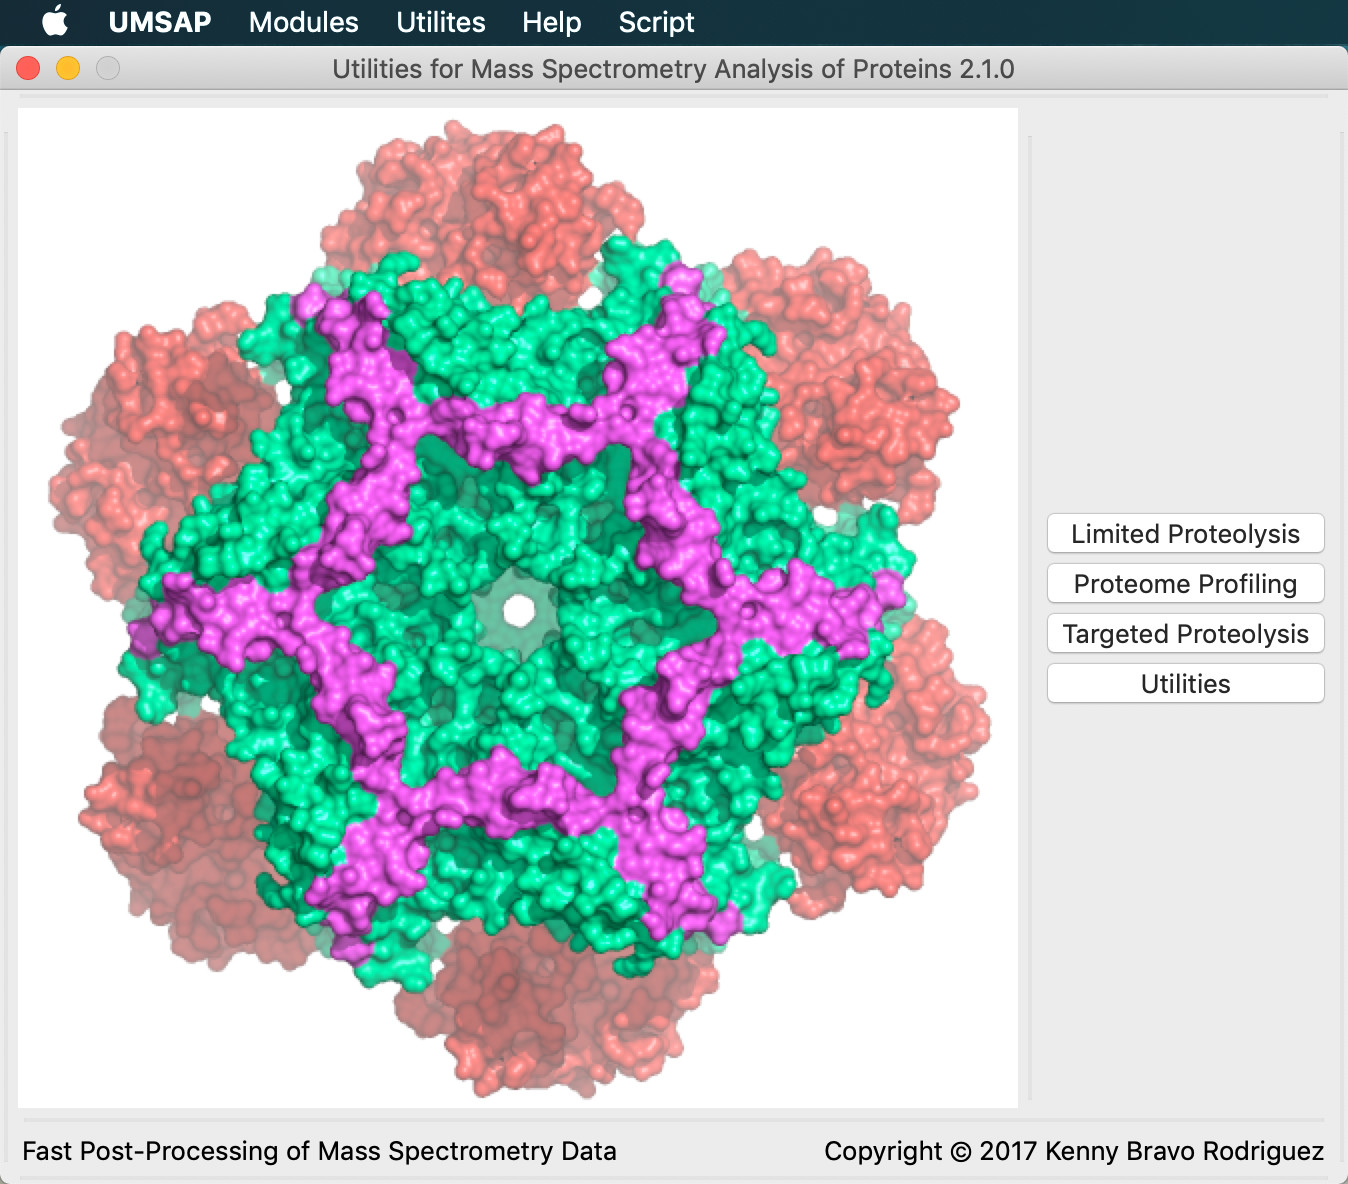
\includegraphics[width=0.7\textwidth]{./IMAGES/MAIN-WINDOW/mainwindow.jpg}	    
	\caption[The main window of UMSAP]{\textbf{The main window of UMSAP.} From this window users can access all the available Modules and Utilities.} 
	\label{fig:mainWindow}
	\vspace{-5pt} 	
\end{figure}  

\section{The input data files}
\label{sec:dataFile}

UMSAP has two main input data files. One file contains the detected peptide sequences after all peak assignments have been completed and the other file contains the detected proteins. The program expects these files to be plain text files containing a table with the data. Columns in the files are expected to be tab separated. The first row in the files is expected to contain only the names of the columns. There is no limitation in the amount and type of data present in the data files. However, each module will expect certain columns to be present. Columns not needed by the modules will simply be ignored.

In addition, certain modules use other input data files as well. The modules Targeted Proteolysis and Limited Proteolysis may use fasta files containing the sequences of the recombinant and native proteins used in the experiments. The fasta files must contain only one protein sequence. Alternatively, instead of a fasta file, a plain text file can be used. In this case, the plain text file must contain only the sequence of a single protein using the one letter code for amino acids. The Targeted Proteolysis module may also use a pdb file. The sequence and pdb files can be directly download from UNIPROT or PDB, respectively,  by supplying the correct codes.

Certain output files generated by UMSAP can be used as input data files as well. Files that can be used this way will contain the results from previous data post-processing. These output files will be plain text files, since in some cases users will need to directly read the data contained in these files. However, it is important that these files remain unchanged to ensure the correct display of the results contained in the files by UMSAP.

\section{Using Utilities for Mass Spectrometry Analysis of Proteins}

Once the input data files are ready to be analyzed, using UMSAP is straightforward. Just open the program and select a module or utility. In the new window, fill in the needed information and hit the Start analysis button in the bottom right corner. Depending on the amount of data and the complexity of the analysis to perform it may take a few minutes for the program to complete the task at hand. In each window performing an analysis, there is a progress bar near the Start analysis button that gives a rough guess of the remaining time needed to complete the current analysis.

Currently, the text boxes showing the path to a file  do not have auto-complete capabilities. In addition, relative paths are not supported. Therefore, the full paths to files are needed. In the case of output files and folders if the text boxes are left empty, appropriate defaults values will be provided, based on the main data file path.  

In order to make the program as user friendly as possible help messages will pop up from buttons and labels. The help messages will contain a brief description of what is the button or label for and what input is expected from the user. In this way, users can find basic information about a particular element of the interface without needing to go to the manual or online tutorials. If more information is needed, users may consult the manual or click the Help button in the bottom left corner of the module/utility window to read an online tutorial. 

Depending on the module or utility just run, new windows will be created to show a graphical representation of the results.

Special care have been taken to handle errors that may appear during the processing of the input files. Errors will be reported to users using dialog boxes with plain English messages so users may correct the errors right away and continue with the analysis. In the case of an unforeseen error occurring, the message error will be more code oriented. It will be helpful if users send a crash report to umsap-crashreport@umsap.nl so we can correct the error and/or create an appropriate error message. 

In general, windows showing a graphical representation of results will be allowed to resize while module/utilities windows will not. The Tools menu will have options specific for each window. In most of the windows the functionalities in the Tools menu can be also accessed with the right mouse button.

\phantomsection
For modules, UMSAP will create a .uscr\label{par:uscrFile} file after finishing the analysis. This is an input file that can be used to run an analysis one more time without users having to type in again all the needed information. Once the .uscr file is selected, using the Run Input File entry in the Script menu, the appropriate module will be launched and the information found in the .uscr file will be used to fill the fields in the interface of the module. At this point, users may decide to update the analysis by changing some of the parameters in the interface of the module. Clicking the Start analysis button will start the analysis of the input data files. More details are given in \autoref{subsec:utilUscrFile}.  

The helper window designed to facilitate the definition of the control and various experiments in each module will try to read the values from a .uscr, .txt file or the given text in the corresponding text entry of a module interface. If something goes wrong while reading the given values, then the helper window will default to show the corresponding empty fields so users can define the experiments and control for the module.

\section{Navigating through Utilities for Mass Spectrometry Analysis of Proteins}

The entries Modules and Utilities will be available in the menu of every window. The Modules entry in the menu gives direct access to all modules. The same is true for the Utilities entry. These menu entries are the fastest way to access all the functions in UMSAP. In a typical UMSAP session, users will work with different independent windows simultaneously. The windows have descriptive names so users can quickly guess the content of any window. The scheme of the windows name is \textit{UMSAP - Utilities or Module Name - Name of the window}. For example, the window with name \textit{UMSAP - Utilities - Correlation coefficients (t\num[detect-all]{1}.corr)} will be displaying the correlation coefficient matrix saved in the file \textit{t\num{1}.corr}.

\subsection{Keyboard shortcuts}

The following table contains the built-in keyboard shortcuts.

\begin{table}[h!]
	\centering
	\begin{tabular}{l l l}
		\hline
		\multicolumn{1}{c}{Shortcut} & \multicolumn{1}{c}{Action} & \multicolumn{1}{c}{Module} \\
		\hline
		Ctrl/Cmd+D & Close current window & All \\		
		Ctrl/Cmd+I  & Read UMSAP .uscr file & All \\		
		Ctrl/Cmd+Q & Quit UMSAP                & All \\
		Ctrl/Cmd+R & Read UMSAP output file  & All \\		
		Alt+Cmd+L & Launch the Limited Proteolysis module & All \\
		Alt+Cmd+P & Launch the Proteome Profiling module  & All \\
		Alt+Cmd+T & Launch the Targeted Proteolysis module & All \\
		Alt+Cmd+U & Launch the Utilities window & All \\		
		Ctrl/Cmd+L & Change selection mode & Limited Proteolysis \\								
		Ctrl/Cmd+Z & Remove last applied filter & Proteome Profiling \\
		\hline		
	\end{tabular}
	\caption[List of built-in keyboard shortcuts]{\textbf{List of built-in keyboard shortcuts.}}
	\label{table:shortcuts}
\end{table}

\section{The output files}

In order to minimize user input, the names for output files and output folders can be left unspecified. In this case, UMSAP will use default names for files and folders. When names for files and folders are given, it is recommended to use names with no spaces, e.g. my-output-file or myoutputfile.The software will avoid to overwrite previous output files or folders. If a selected folder already exists and it is not empty, UMSAP will create a new folder to write in the results. The location of the new folder will be the same as the selected folder. The name of the new folder will be the same as the selected folder plus the current date and time to the second, for example, selectedfolder-20190425092904. The same is true for files unless the user forces UMSAP to overwrite a file. 

In general, the output file will be saved using a json format. If needed the data can be exported to a csv format with tab delimited columns, see \autoref{subsec:utilExpData}. 

\section{Backward compatibility}
\label{sec:backwardCompatibility}

UMSAP is capable to read the .tarprot file from previous versions. Other files generated by UMSAP are version dependent and cannot be read in with different versions of UMSAP. Nevertheless, two tools allows to quickly generate any UMSAP file based on a .tarprot file from a previous version of UMSAP. These tools are described in \autoref{subsec:utilUpdateRes} and \autoref{subsec:utilReanalyzeTarprot}. How to generate a .tarprot file is explained in \autoref{chap:tarprot}.